\subsection{Brassinoslide Component}

\cite{vukasinovic2021} provide a detailed biosynthetic pathway for BL, which is presented in Figure \ref{fig:biosynthetic-pathway}. Since BL is the most biochemically active brassinosteroid \cite{vanesse2012}, we will assume that it is only brassinosteroid when modelling. 

\begin{figure}[!htbp]
    \centering
    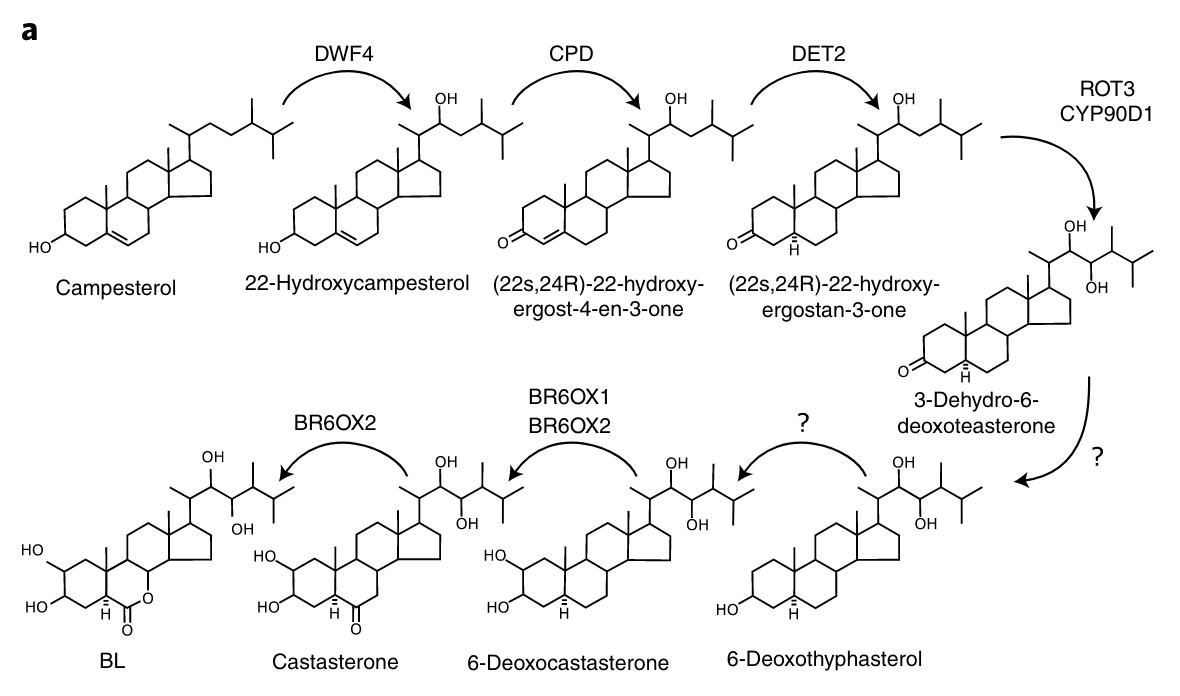
\includegraphics[width=13cm]{img/brassinosteroid-precursors.png}
    \caption{Biosynthetic pathway leading to the formation of BL from campesterol. Mutants deficient in each of the enzymes shown above the transition arrows (DWF4, CPD, DET2, etc.) exhibited stunted growth (\cite{vukasinovic2021}).}
    \label{fig:biosynthetic-pathway}
\end{figure}

\medskip

The biosynthetic enzymes CPD and ROT3 were observed by \cite{vukasinovic2021} using fluorescence imaging in the vascular cell columns of a single root. Their results are shown in Figure \ref{fig:cpd-rot3-levels}.

\begin{figure}[!htbp]
    \centering
    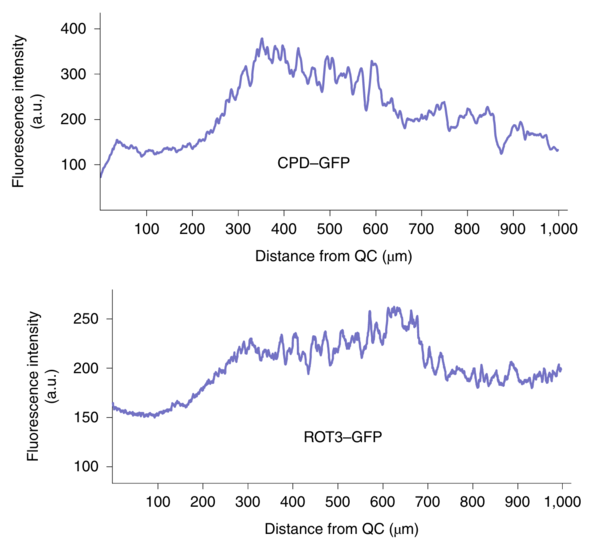
\includegraphics[width=13cm]{img/cpd-rot3.png}
    \caption{The levels of CPD and ROT3 remain relatively constant in the meristem (0-200\um) before increasing in the transition zone (200-400\um) and reaching a maximum in the elongation zone (400-700\um) (\cite{vukasinovic2021}).}
    \label{fig:cpd-rot3-levels}
\end{figure}

\medskip

We make the assumption that the fluorescence intensity of CPD and ROT3 correspond to the concentration of BL ligand up to some scalar multiple.  To determine this scalar, we use an estimate from \cite{vanesse2012} that gives the extracellular concentration of BL ligand to be at most 1\nm in wild-type roots. This gives us the following formula for the extracellular BL concentration [BL] in \nm:


\begin{equation}
    \label{bl}
[\text{BL}] = b \cdot \frac{\text{CPD}}{\text{max}(\text{CPD})} + (1 - b) \cdot \frac{\text{ROT3}}{\text{max}(\text{ROT3})}
\end{equation}

\medskip

In \eqref{bl}, the parameter $b \in [0, 1]$ controls the bias towards CPD in order to account for the fact that the exact details of the BL pathway are omitted from our model. Using the data from Figure \ref{fig:cpd-rot3-levels} along with \eqref{bl}, we get the plot of BL concentration against position shown in Figure \ref{fig:bl-bias}.

\begin{figure}[!htbp]
    \centering
    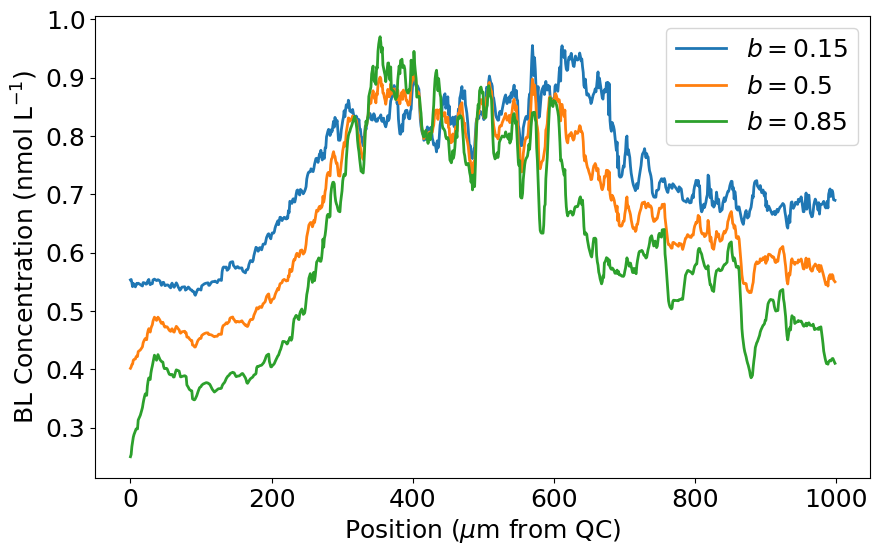
\includegraphics[width=13cm]{img/bl-bias.png}
    \caption{The BL concentration function for three different values of the bias parameter $b$. For future simulations we will use $b = 0.5$, since the BL concentration function exhibits similar qualitative behaviour for all $b$ as shown above.}
    \label{fig:bl-bias}
\end{figure}

\medskip

Additionally, BR biosynthetic enzymes have been shown to move short distances in the root (\cite{vukasinovic2021}), so we take an $n\,\um$ moving average of the BL concentration function to account for diffusion. Shown in Figure \ref{fig:bl-average} is a plot of the BL concentration function after the moving average has been applied to the CPD and ROT3 functions.

\begin{figure}[!htbp]
    \centering
    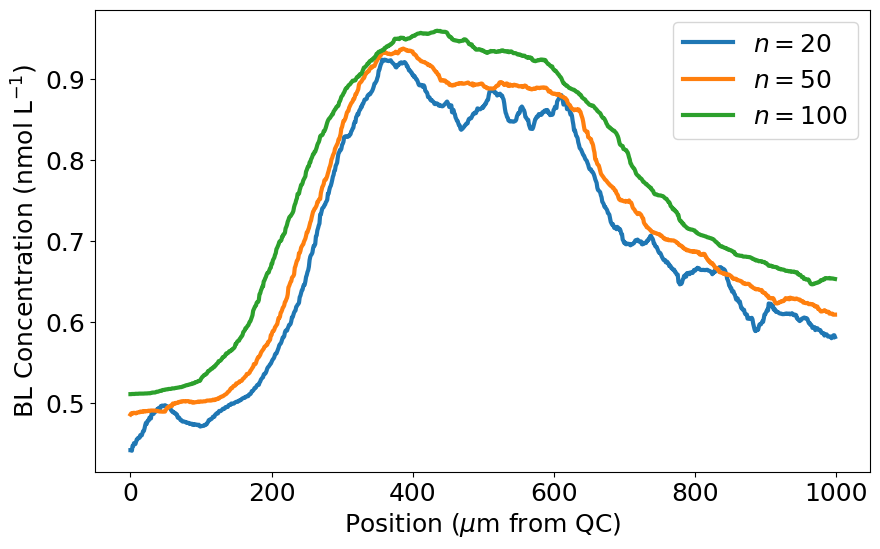
\includegraphics[width=13cm]{img/bl-average.png}
    \caption{A plot of BL concentration functions ($b = 0.5$) for three different values of the moving average period $n$. Future simulations will use $n = 50$, an admittedly arbitrary choice since the exact details of the diffusive effect we are modelling are unknown.}
    \label{fig:bl-average}
\end{figure}


